% Pacotes e configurações padrão do estilo ``article''\
% -------------------------------------
\documentclass[a4paper,11pt]{article}
% Layout
% ------------------------------------------------------------------------------
%     Gráficos e layout ----------------------------------------------------------------------

\ifx\pdfmatch\undefined
\else
    \usepackage[T1]{fontenc}
    \usepackage[utf8]{inputenc}
\fi
% xetex:
\ifx\XeTeXinterchartoks\undefined
\else
    \usepackage{fontspec}
    \defaultfontfeatures{Ligatures=TeX}
\fi
% luatex:
\ifx\directlua\undefined
\else
    \usepackage{fontspec}
\fi
% End engine-specific settings

%      Fonte --------------------------------------------------------------------------------
%\usepackage{lmodern}
\usepackage{times}
%     Pacotes adicionados -------------------------------------------------------------------
\usepackage{ae}
%     Língua e hifenização ------------------------------------------------------------------
\usepackage[portuguese]{babel}
\usepackage{hyphenat}
%      Outros --------------------------------------------------------------------------------
\usepackage{hyperref} % Permite Links personalisados usando hyperref
\usepackage{fancyhdr}
\usepackage{sectsty}
\usepackage{float}   % Gerencia melhor o posicionamento das figuras e tabelas
%\usepackage{graphicx}
\usepackage[pdftex]{color,graphicx}
\usepackage{hyperref}
\usepackage{enumerate} % Permite alterar Layout do enumerate
%\usepackage{pdflscape}  % Permite alterar a orientação da pagina para Paisagem
%\usepackage{ifthen}  % Permite usar condicionais ifelse
%\usepackage[table]{xcolor} % Permite alterar as cores das células de uma tabela
\usepackage{amsmath,amssymb} % Ambiente para uso de elementos matemáticos
\usepackage{caption}
\usepackage{subcaption} % permite o uso de multiplas figuras com legenda (ambiente subfigure)
\usepackage{minted} % Ambiente minted para colorir código de programas
\usepackage{natbib} % Para referencia bibliográfica
\usepackage{url}    % Referência de links na internet
%\usepackage{listings} % pacote para apresentar código de programação
\usepackage{indentfirst}  % Para indentar o primeiro parágrafo de cada seção
\usepackage{titling}  % Permite Montar uma página de titulo própria

% Layout do documento ------------------------------------------------------------------------
%     Bordas e tamanho da página ------------------------------------------------------------
\usepackage{geometry} 
 \geometry{ % Padrõa ABNT para relatórios
 a4paper,
 left=30mm,
 right=20mm,
 top=30mm,
 bottom=20mm
 }
%     Cabeçalho e Rodapé ---------------------------------------------------------------
\pagestyle{fancy}
  \lhead{}
  \chead{}
  \rhead{}
  \lfoot{}
  \cfoot{}
  \rfoot{\thepage}
%     Númeração ------------------------------------------------------------------------
  \pagenumbering{arabic}
%     Retas do cabeçalho e rodapé ------------------------------------------------------
  \renewcommand{\headrulewidth}{0.5pt}
  \renewcommand{\footrulewidth}{0.5pt}
%     Tamanho da letra de seções e derivadas --------------------------------------------
  \sectionfont{\normalsize}
  \subsectionfont{\small}
%     Hiperlinks ------------------------------------------------------------------------
  \hypersetup{
                  colorlinks,
                  citecolor=black,
                  filecolor=black,
                  linkcolor=black,
                  urlcolor=black
                  }
%     Definições do pdf ----------------------------------------------------------------------
\hypersetup{
    unicode=false,          % non-Latin characters in Acrobat’s bookmarks
    pdftoolbar=true,        % show Acrobat’s toolbar?
    pdfmenubar=true,        % show Acrobat’s menu?
    pdffitwindow=false,     % window fit to page when opened
    pdfstartview={FitH},    % fits the width of the page to the window    
    pdfauthor={Rafael Lima},     % author
    pdfnewwindow=true      % links in new window
}
%     Outros ----------------------------------------------------------------------------
      %\renewcommand{\thesection}{(\alph{section})} % muda o estilo de númeração das sections
      % alterando a formatação dos numeradores de lista de itens
      \renewcommand\theenumi{\arabic{enumi}}
      \renewcommand\labelenumi{(\textit{\theenumi})}
	  \renewcommand\theenumii{\arabic{enumii}}
	  \renewcommand\labelenumii{(\textit{\theenumi.\theenumii})}
      
% ---------------------------------------------------------------------------------------


\usepackage{tikz}
\usetikzlibrary{arrows,shapes,automata,petri,positioning}

%\usepackage{circuitikz}

\title{Projeto - Controle a Evento discretos} % Define o título do Relatório
\author{Rafael Lima}

% Definições Auxiliares ( Macros próprias )
% ------------------------------------------------------------------------------
%\input{relat_aux.tex} % Arquivo com minhas macros
\tikzset{
    place/.style={
        circle,
        thick,
        draw=blue!75,
        fill=blue!20,
        minimum size=6mm,
    },
    transitionH/.style={
        rectangle,
        thick,
        fill=black,
        minimum width=8mm,
        inner ysep=2pt
    },
    transitionV/.style={
        rectangle,
        thick,
        fill=black,
        minimum height=8mm,
        inner xsep=2pt
    }
}
% ----------------------------------~>ø<~---------------------------------------
\begin{document}
% Capa e Índice ----------------------------------------------------------------
%--------------------------------------------------- Capa --------------------------------------------
%\newpage
\begin{figure}[h!]
\centering

\includegraphics[scale=0.9]{img/simb_unb.png}
\label{fig:unb}
\end{figure}

\begin{center}
{\LARGE Universidade de Brasília}\\
Departamento de Engenharia Elétrica\\
Professor: Fernando\\
Disciplina: Controle para Automação\\
\end{center}

\vspace{0.18\textheight}

\begin{center}
    \Huge \textbf{\\\thetitle \\}
\end{center}

\vspace*{\fill} % Completa espaço em branco e empurra o resto para o final da página

% Tabela com os nome das pessoas do grupo

\begin{table}[H]
    \begin{tabular}{ll}
        % Nome      & Matrícula
        Rafael Lima & 10/0131093 \\
    \end{tabular}
\end{table}

\vspace{0.5cm}

\begin{center}
    \textbf{Brasília\\
    \the\year} % Coloca o Ano atual
\end{center}

\thispagestyle{empty} % Retira o cabeçalho e o rodapé da página

% ------------------------------------------------- Índice -------------------------------------------
\newpage
\tableofcontents
\newpage
% ----------------------------------------------------------------------------------------------------

 % Capa para UnB
% Conteúdo ---------------------------------------------------------------------

\section{Objetivos}

Implementação de sistema automático para controle de nível de um buffer em que é acionado um motor de forma automática quando for detectado que o mesmo esteja vazio.

\section{Desenvolvimento}

\subsection{Modelagem por Máquina de Estados Finitos}

\subsubsection{Levantamento Estados e Eventos}

A partir da descrição do sistema proposto temos as seguintes entradas e acionamentos

\begin{itemize}
    \item Acionamentos
    \begin{itemize}
        \item Motor ( Desligar, Giro em sentido horário e Giro em Sentido Anti-horário )
        \item Sinalização Motor: Duas Luzes
        \item Sinalização Buffer: Duas Luzes
    \end{itemize}
    \item Entradas
    \begin{itemize}
        \item Botoeira Liga
        \item Botoeira Desliga
        \item Botoeira Parada de Emergência
        \item Sensor de Nível
        \item Chave Seletora para o sentido do Motor
    \end{itemize}
\end{itemize}

A partir desta descrição foi adotado a modelagem por máquina de estados. Cada alterações no estado dos dispositivos de entrada foi associado a um evento e os conjunto de comandos nos dispositivos de Acionamentos referente a uma ação do sistema foram agrupados como estados.

Do ponto de vista de comportamento macro do sistema podemos descrever o sistema seguinte forma:

\begin{table}[H]
    \centering
    \begin{tabular}{c|cc}
        \hline
        Estado & $L_{s_2}$ & $S_{nivel}$ \\
        \hline
        Desligado & Desligado & - \\
        Buffer Cheio & Desligado & $1$\\
        Buffer Vazio & Piscando & $1$\\
        \hline
    \end{tabular}
    \caption{Caption}
    \label{tab:states_buffer}
\end{table}

A partir da tabela \ref{tab:states_buffer} podemos representar o comportamento buffer associado a leitura do sensor como

\begin{figure}[H]
    \centering
    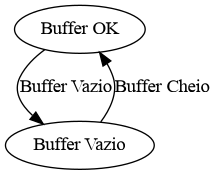
\includegraphics[width=0.6\linewidth]{src/tex/img/automato_buffer.png}
    \caption{Caption}
    \label{fig:automato_buffer}
\end{figure}

Por outro lado do ponto de vista de controle do motor temos:

\begin{table}[H]
    \centering
    \begin{tabular}{c|cccl}
        \hline
        Estado & $L_{s_1}$ & $L_{m_1}$ & $L_{m_2}$ & Motor \\
        \hline
        Motor Desligado & $0$ & $0$ & $0$ & Desligado\\
        Ligado Sentido Horário & $1$ & $1$ & $0$ & Desligado\\
        Ligado Sentido Anti-Horário & $1$ & $0$ & $1$ & Desligado\\
    \end{tabular}
    \caption{Caption}
    \label{tab:states_motor}
\end{table}

A partir da tabela \ref{tab:states_motor} podemos o comportamento desejado do motor como

\begin{figure}[H]
    \centering
    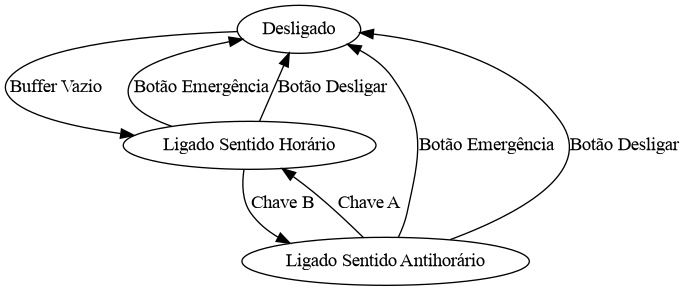
\includegraphics[width=0.9\linewidth]{src/tex/img/automato_motor.png}
    \caption{Caption}
    \label{fig:automato_motor}
\end{figure}

\subsection{Modelagem por Rede de Petri}

\begin{figure}
    \centering
    \begin{tikzpicture}[node distance=0.5cm and 1cm,>=stealth',bend angle=45,auto]
        \node [place,label=above:$P_1$] (p1) {};
        \node [transitionV,label=above:$T_1$] (t1) [right= of p1] {}
            edge[name=t1]   (p1);
        \node [place,tokens=1,label=above:$P_2$] (p2) [above right=of t1] {}
            edge[pre]   (t1);
        \node [place,tokens=2,label=above:$P_3$] (p3) [below right=of t1] {}
            edge[pre]   (t1);
        \node [transitionV,label=above:$T_2$] (t2) [above right=of p3] {}
            edge[pre]   (p2)
            edge[pre]   (p3)
            edge[post,out=-110,in=-50,looseness=2,overlay]  (p1);
        \node [place,tokens=1, label=above:$P_4$] (p4) [above right=of t2] {}
            edge[pre]   (t2);
    \end{tikzpicture}
    \caption{Caption}
    \label{fig:my_label}
\end{figure}

\subsection{Modelagem em Ladder}

\section{Conclusão}

% ------------------------------------------------------------------------------
\newpage
% Referências
\addcontentsline{toc}{section}{Referências} % Adiciona linha no índice
\bibliographystyle{abbrv} % Define Estilo e gera bibliografia
\bibliography{references} % Adiciona Arquivo com Referências

% Acrescentadas no arquivo references.bib
% para usa-las no texto basta usar \citep{}
% para citar sem usar no texto basta usar \nocite{}
%\nocite{sympy}
%\nocite{pythontex}
%\nocite{matlabcontrol}
%\nocite{matlabsymbolic}
%\nocite{ogata2010modern}
%\nocite{nise2012}

% ------------------------------------------------------------------------------
\newpage
\section*{Anexos}
\addcontentsline{toc}{section}{Anexos} % Adiciona linha no indice
%\subsection*{Python}

%Para os cálculos e demonstrações foi utilizado o pacote \textit{Python}\TeX\ \cite{pythontex} para o \LaTeX\ em conjunto da bibliteca \textit{sympy}\cite{sympy}. Segue o script completo em python:

%\inputminted[xleftmargin=15pt,linenos,frame=single,framesep=5pt,breaklines=true]{python}{../python/exsim6.py}

%\newpage
\subsection*{Matlab}

Foi utilizado o \textit{Matlab} em conjunto da toolbox\textit{Symbolic Math}\cite{matlabsymbolic}. Para facilitar o estudo de forma interativa, o código foi dividido em múltiplos arquivos contendo funções auxiliares e um arquivo de script contendo todo a lógica usada para gerar as figuras e diagramas

\subsubsection*{Script Principal}

\inputminted[xleftmargin=15pt,linenos,frame=single,framesep=5pt,breaklines=true]{matlab}{../matlab/petrinetproject.m}

\subsubsection*{Funções Auxiliares}

Inicialmente foi definido uma função para verificar se uma transição é permitida para um determinado estado:

\inputminted[xleftmargin=15pt,linenos,frame=single,framesep=5pt,breaklines=true]{matlab}{../matlab/petristate.m}

Para avaliar as transições da Rede de Petri foi definido uma função auxiliar para gerar as árvores de transição de estados:

\inputminted[xleftmargin=15pt,linenos,frame=single,framesep=5pt,breaklines=true]{matlab}{../matlab/dotpetree.m}

% ------------------------------------------------------------------------------
\end{document}
